% Documentation:
%
% The UoK class file extends the standard report style to follow the Registry
% guidelines for laying out a thesis. It sets the margins, interline spacing,
% the page, figure and table numbering style, and disallows page breaks at
% hyphens. The class file consists of setting one and an half line spacing text
% with a 4cm left margin, at least a 2.5cm right margin, approximately 2cm top
% and bottom margin, on A4 paper.
% 
% The class the following options, in addition to those of the standard report
% class.
%     mini - Toggles the thesis in to mini-thesis mode. This adds "mini" to the
%            title and appends a nocite(*) at the end for an automatic output of
%            your complete bibliography.
%     draftmark - Puts a DRAFT' watermark on every page of the document along
%                 with the draft statement on the title page. Additionaly, it
%                 is used as a switch for the UoKExtentions package.
%     draft - Puts the entire document into draft mode. Applies all the effect
%             of draftmark above, but also propergates to other packages used.
%     copyright - Adds a copyright page between the title page and the preface.
%     nofig - Disables output of the list of figures in the preface.
%     notab - Disables output of the list of tables in the preface.
% All options passed to UoKthesis will be passed along to included packages:
%    natbib, draftwatermark, setspace, hyperref, lmodern
%
% The cover page and optional copyright page are implicitly added before the
% start of the preface section. Use the following commands to populate the 
% cover page/copyright page information:
%     \title{thesis title}
%     \author{author's name} 
%     \degree{Master of Science, Doctor of Philosophy, etc.} 
%     \subject{author's department}
%          - Computer Science if omitted 
%     \submitdate{month year in which submitted}
%          - dated by LaTeX if omitted 
%     \copyrightyear{year degree conferred (next year if submitted in Dec.)}
%          - assumes current year (or next year, in December) if omitted 
% 
% The preface environment allows for the use of sections that precede the main
% document; such as Abstract and  Acknowlegements. These sections should be
% defined using \section{Preface Section Title}. The contents page (and list of
% figures and tables if in use) will be automatically inserted at the end of the
% preface environment.
%
% The thesis style invokes the setspace package to set the commands:
%     \doublespace
%     \onehalfspace
%     \singlespace
% for spacing. By default one and an half spacing is used which resembles the
% UKC Typewriter requirement. Singlespace can be used for letterpress
% appearance. If you want to use true double space, for some reason, place the
% \doublespace command where you want to start using double spacing. Just call
% the appropriate spacing command at where you want to use them.
% 
% In the figure and table environments, single spacing is used. If you want to
% use any other size rather than one and an half spacing, then do:
% 	\renewcommand{\baselinestretch}{1.6} (or whatever you want instead of 1.6)
% This command won't take effect unless it comes before the \begin{document} or
% is triggered by a font change (after something like \small \normalsize).
%
% The example below shows the 12pt thesis style being used. This seems to give
% acceptable looking results, but it may be omitted to get 10pt. Alternatively,
% the 11pt option can be used.
%
% This version differs from old_ukcthesis.sty in the following ways:
% 1. Removed the doublespace package (now uses setspace).
% 2. Merged the phantom section for correct PDF links into the bibliography
%    generating function. 
% 3. Added thesis type options (mini, draft).
% 4. Kent Harvard is used for referencing and citation, this is supported by the
%    natbib package.
% 5. PsFig macro removed.
% 6. Now comes as two files, UoKthesis.cls, which defines purely stylistic layout,
%    and UoKextentions.sty, that provideds some additional functionality.

\documentclass[12pt]{UoKthesis}

%\renewcommand*\rmdefault{ptm}
%\renewcommand{\familydefault}{\rmdefault}
% Note: The UoKextentions package includes the xcolor package with the [usenames]
% options. If you need to add further options, these can be given to UoKextentions
% to be propogated through.
\usepackage{UoKextentions}
\usepackage{times}
%\usepackage{llncsdoc}
%\usepackage{verbatim}
\usepackage{url}
\usepackage{color}
\usepackage{amsmath}
\usepackage{relsize}
\usepackage[final]{listings}
\usepackage[T1]{fontenc}
%\usepackage[math]{times}
\usepackage{mathptmx}
\usepackage{graphicx}
\usepackage{wrapfig}
\usepackage[scaled=.90]{helvet}
\usepackage{courier}
\newcommand{\td}[1]{{\bf {\tt{#1}}}}
\newcommand{\comment}[1]{\textcolor{red}{\td{{#1}}}}
\usepackage{textcomp}
\lstset{
  frame=none,
  xleftmargin=2pt,
  stepnumber=1,
  numbers=left,
  numbersep=5pt,
  numberstyle=\ttfamily\tiny\color[gray]{0.3},
  belowcaptionskip=\bigskipamount,
  captionpos=b,
  escapeinside={*'}{'*},
  language=haskell,
  tabsize=2,
  emphstyle={\bf},
  commentstyle=\it,
  stringstyle=\mdseries\ttfamily,
  showspaces=false,
  keywordstyle=\bfseries\ttfamily,
  columns=flexible,
  upquote=true,
  showstringspaces=false,
  basicstyle=\small\ttfamily,
  breaklines=true,
  morecomment=[l]\%,
}

% Kent Harvard Bibliography Style. WIP
\bibliographystyle{kentHarvard}

% Provides nice linking in PDFs
\usepackage{hyperref}

% Only needed if you want to produce an index. Example is shown at the bottom of this document.
\usepackage{makeidx}

% Useful packages
% \usepackage{epstopdf} % Converts EPS files to PDF using ghostscript
% \usepackage{fnbreak}  % Warns you if you have split footnotes
% \usepackage{mathpazo} % Type­set­ math­e­mat­ics in the Palatino fam­ily of text fonts
% \usepackage{paralist} % Enumerate and itemize within paragraphs
% \usepackage{amsmath}  % AMS mathematical facilities
% \usepackage{rotating} % Rotating facilities for floats


\setcounter{secnumdepth}{3} % add more section types

%%%%% macros
\def\fixme#1{\fbox{\textbf{\textsc{Fixme}}\quad#1}}
\def\fixpic#1{\fbox{\textbf{\textsc{Picture}}\quad#1}}
\def\defnx#1#2{\emph{#1}\index{#2}}
\def\defn#1{\defnx{#1}{#1}}
\def\floatpic#1#2{%
\begin{wrapfigure}{r}{\dimexpr #1 / 2 \relax}
\includegraphics[width=\dimexpr #1 / 2 \relax]{#2}
\end{wrapfigure}}
\def\inlinepic#1#2{%
\begin{center}
\includegraphics[width=\dimexpr #1 / 2 \relax]{#2}
\end{center}}

%%%%% augment hyphenation
\hyphenation{wide-spread}

%%%%% document start
\begin{document}

\title{Type-Changing Refactorings in Haskell}
\author{Stephen Adams}
\subject{Computer Science}
\degree{PhD}

\begin{preface}
\section{Abstract}
This mini-thesis tells you all you need to know about...
\section{Acknowledgements}
I would like to thank...
\end{preface}

\chapter{Introduction}\label{chp:intro}


\section{Functional Programming}
Functional programming is a programming paradigm that focuses on data values as described by expressions which are built from function applications and definitions~\citep{elementsOfFunc}.  Functions in this case are closely related to the idea of mathematical functions. Another key concept of a functional programming language is that functions are \textit{first class citizens}. This means that functions can be used like any other type of data, e.g. as arguments to other functions. 
  
\section{Haskell}
Haskell is a statically typed, lazily evaluated, pure functional language. Haskell is strongly and statically typed, and supports Hindley-Milner type inference~\citep{wikiIntro}. Type inference means that a Haskell programs do not need every type to be explicitly listed in the source code. Types will be~\textit{inferred} at compilation time so that every part of a Haskell program's type is known at that time. Haskell's type system also allows users to define their own types.

Lazy evaluation means that Haskell expressions are not evaluated when they are passes as a parameter, but rather when that value is used. For example in the Haskell function:
\clearpage
\begin{verbatim}
f x y = case x > 0 of
True -> x - 1
False -> x + 1
\end{verbatim}

The parameter y will never be evaluated.

Haskell is also a pure language. Purity is the idea that functions cannot perform actions in addition to returning values. These additional actions are known as side-effects. Haskell allows for traditionally side-effect causing operations (IO, state, etc.) through the use of monads. Monads contain any potentially side effect causing operations inside of them allowing the rest of the program to remain pure.

\section{Refactoring} 
Refactoring is the process of changing a program without changing its behaviour. This is done to improve its internal structure~\citep{fowler}. Behaviour preservation is what separates refactoring from other types of program manipulation. This idea of functionality preservation means that refactoring will not introduce new bugs or eliminate old ones. To prevent semantic changes after refactoring, many refactorings have non-trivial preconditions~\citep{refacTools}. 

Manual refactoring is tedious and error prone, and depends on high testing coverage to ensure that functionality is preserved~\citep{fowler}. This means that tools that can automatically perform refactorings and ensure that preconditions are met are highly desirable.

\subsection{Functional refactoring}

Refactoring a functional language has a few key differences from refactoring an imperative language. The higher-order nature functional languages means that any sub-expression of a function is a candidate for generalisation whereas in other languages the types of parameters and results is limited. The semantics of functional languages also allow for the complete checking of preconditions based on the static semantics of the language~\citep{refacTools}.

It is also not unusual for functional refactorings to be substantially different than their object-oriented (OO) counterparts. For example creating a case statement from a multi-equation function definition in a functional language versus inlining a virtual method as a case statement in an OO language require substantially different program manipulations~\citep{huiqingThesis}. Additionally there can be refactorings with no OO counterpart, monadification, for instance.  

\section{Contributions of this Research}

\comment{TODO}

\section{Thesis Outline}

\comment{TODO}


\chapter{Background: Refactoring Haskell in HaRe}
\label{hare}

\comment{
Chapter~\ref{hare} is where the development and implementation of HaRe will be discussed. The chapter with cover some of the history or HaRe and the briefly the technology that it was originally developed with. Next it will cover the design and implementation of HaRe currently and its dependencies (in particular ghc-exactprint). }

\td{
A brief outline of this chapter:

\begin{enumerate}
\item The original implementation of HaRe
\item The GHC API
\item Generic Programming (Scrap Your Boilerplate and Strafunski-StrategyLib)
\item GHC-ExactPrint
\item The Current version of HaRe
\end{enumerate}
}

Work on creating the refactoring tool HaRe started in early 2003 at the University of Kent and was originally worked on by Huiqing Li, Claus Reinke, and Simon Thompson~\citep{refacWebsite}. This chapter will start with a brief discussion of this original implementation. The Haskell ecosystem that the original HaRe supported is very different from the Haskell ecosystem that most Haskell programmers use today. HaRe was originally implemented to support the Haskel 98 standard~\citep{huiqingThesis}. However, the Glasgow Haskell Compiler (GHC) has now become the de facto Haskell standard~\citep{refacTools} and HaRe has been updated to support the GHC. The second half of this chapter will describe the current implementation of HaRe and the major dependencies that it uses. 

\section{The original implementation of HaRe}

Implementing an automated refactoring system requires several dependencies, a frontend for the language that you are targeting, a generic programming library, and a pretty printer. The language frontend is required for your refactorer to analyse and modify source code, the generic programming library assists in traversing the complex abstract syntax tree of a real world programming language, and the pretty printer outputs the modified AST. The original implementation of HaRe fulfilled these dependencies with two libraries, Programatica and Strafunski-StrategyLib. 

\subsection{Programatica and Strafunski}\label{prog&Strafunski}

Programatica was a project at the OGI School of Science and Engineering to build tool support for validating Haskell programs~\cite{programaticaTools}. The Programatica team open sourced their frontend so that other tools could also use it~\citep{refacWebsite}. HaRe chose to use Programatica over other available front ends because it supported the full Haskell 98 standard along with a number of its extensions~\citep{huiqingThesis}. Programatica's Haskell front end is broken up into multiple components including a lexer, a parser, an abstract syntax, a module system, a type checker, and a pretty printer. Programatica's frontend allows for HaRe to focus on refactoring only rather than having to build all of these components as well.

Proogramatica's abstract syntax contains 20 data types with 110 data constructors in total. Working with the syntax directly would introduce a large amount of ``boilerplate" code into HaRe that would make maintenance and reusability of much more difficult~\citep{huiqingThesis}. Instead HaRe used Strafunski-StrategyLib a generic programming to traverse the abstract syntax tree (AST) of the source code. Strafunski-StrategyLib is a combinator library for generic programming~\citep{strafunski}. 

Transforming a program often only modifies small sections of the source program's AST at one time. Renaming a function, for example, will only need to modify the name used in the binding and places where that name is being used, all other sections of the AST remain unmodified. Strafunski takes code that works only on a few data constructors\footnote{In the renaming example this could be code that checks if a variable is the one being renamed and replacing it with the new name.} and ``extends" it to work with every type in the AST. Strafunski also provides ``strategies" that define how that extended function will be applied to the syntax tree~\citep{strafunski}\footnote{e.g. top-down or bottom-up}.

These two dependencies allowed the original implementation of HaRe to obtain the abstract syntax tree of source code to be refactored, traverse and transform that AST, and output the modified program. All these tasks are still things that HaRe needs to do but the dependencies that it relies on have changed somewhat. The Haskell standard was updated in 2010~\citep{haskell2010} and GHC continues to expand the number of language extensions it supports. Unfortunately Programatica has not kept up with these changes and does not support anything beyond Haskell98. At the same time GHC's own API has matured. HaRe now relies on this and a few other projects for its language frontend. For generic traversals Scrap Your Boilerplate has been added as a dependency though Strafunski-StrategyLib is still used.
 
\subsection{HaRe's original refactorings}\label{origRefactorings}

HaRe's original refactorings fall into three categories, structural, module, and data-oriented refactorings.

\subsubsection{Structural Refactorings}

Structural refactorings mainly concern the name and scope of entities defined in a program~\citep{huiqingThesis}. These refactorings tend to modify functions, and smaller, sections of code. A traditional example of this is the renaming refactoring. 

Renaming is one of the most basic refactorings. The purpose of renaming is to change the name of a given identifier. This allows for the way in which you refer to your code to easily stay up to date with what your code actually does. 

Other examples of structural refactorings include delete a definition, duplicate a function, and add an argument~\citep{huiqingThesis}.

\subsubsection{Module Refactorings}

Module refactorings are those refactorings that concern the imports and exports of individual modules, or the relocation of definitions between modules~\citep{huiqingThesis}. A simple refactoring in this category would be ``clean an import list," which analyses a module's import list and removes redundant import declarations. Another example of a refactoring in this category would be the ``move a definition" refactoring. As its name suggests, move a definition takes a definition from one module and moves it to another.

\subsubsection{Data Type Based Refactorings}

The third category of refactorings are those that are associated with data type definitions~\citep{huiqingThesis}. ``Add field names" is a good example of a data-oriented refactoring.  The add field names refactoring will add field names to a data type. These names can then be used as selector functions that make extraction of a particular part of a type a simple function call. The new field names are generated by HaRe but can be renamed by the user~\citep{huiqingThesis}.

These original refactorings were chosen to be basic yet still useful, and for their ability to give insight into the issues surrounding implementing an automated refactoring tool~\citep{huiqingThesis}. In addition to the refactorings that were implemented by HaRe's developers an API was exposed so that other developers could implement their own refactorings~\citep{hareApi}.


\subsection{HaRe's API}\label{hareApi}

Early in the development cycle of HaRe it was restructured to expose an API for implementing refactorings and general Haskell program transformations~\citep{hareApi}. HaRe's API contains a collection of functions for program analysis and transformation of Haskell 98 programs. These functions along with the functionality provided by Strafunski and Programatica form the basis for implementing basic refactorings~\citep{hareApi}.

The HaRe API exposes the full Programatica abstract syntax for Haskell 98 to the user but with the generic programming provided by Strafunski only small sections of the AST need to be dealt with~\citep{hareApi}. Another key feature of the API was to hide layout and comment preservation allowing the programmer to focus on program transformation instead. This is done by having the API's transformation functions modify the token stream and the AST simultaneously~\citep{hareApi}. 

The overall goal of the HaRe API is to help ensure the correctness of new refactorings by limiting the amount of code required that is not related to program transformation and isolating common error sources~\citep{hareApi}. This design goal still guides development of HaRe, and many of the functions that were provided in the original HaRe API have been updated to HaRe's latest incarnation. 
 
\section{The Current Implementation of HaRe}

As was mentioned in subsection~\ref{prog&Strafunski} HaRe's dependencies have changed somewhat in its current implementation. In particular the language frontend is composed of several projects now, the GHC API, ghc-mod, and ghc-exactprint~\citep{ghcApi,ghcMod,exactprint}. This section will describe these new dependencies as well as Scrap Your Boilerplate~\citep{syb}, another generic programming library, and how HaRe currently uses them.

\subsection{The GHC API}

Rather than being a monolithic executable the GHC is composed of several smaller components that each correspond to a separate compiler stage. The GHC executable is just a lightweight main function that ties together the smaller components~\citep{ghcDesign}. These components are exposed to users  and this is what constitutes the GHC API.

\subsubsection{Compiler stages of the GHC}\label{ghcStages}

Some of the major components and the order that the GHC uses them is show in figure~\ref{compilerStages}. This figure is not a complete list of all the components the GHC uses just the parts that HaRe interacts with. The full diagram can be found in~\citep{ghcDesign}. The label after each compiler stage indicates the type of AST that is produced by that stage.

\begin{wrapfigure}{L}{0.5\textwidth}\label{compilerStages}
	\begin{center}
		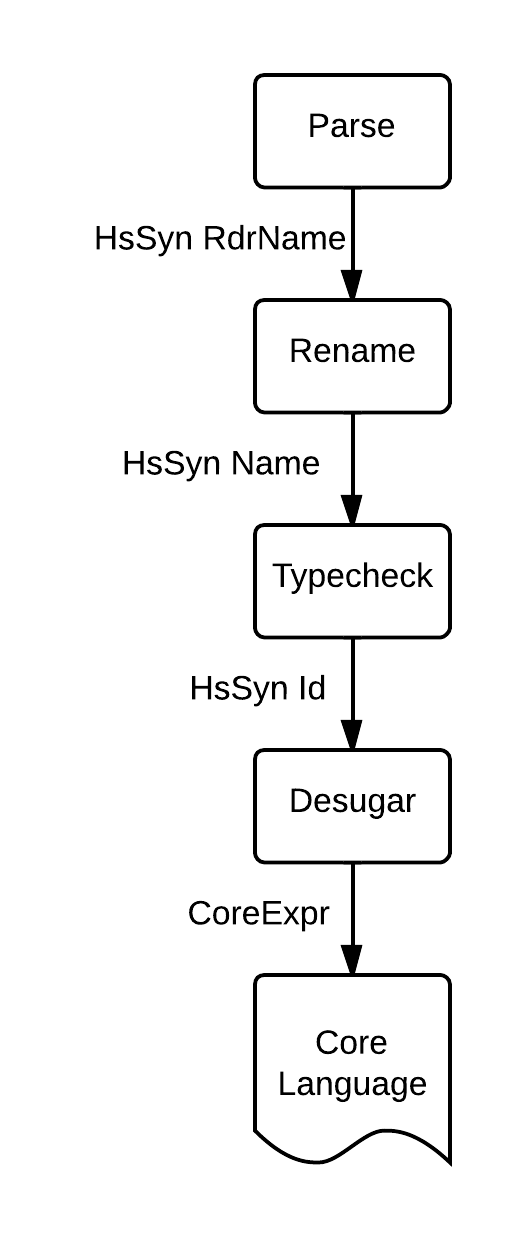
\includegraphics[scale=.3]{images/compilerStages.png}
	\end{center}
	\caption{GHC Compiler stages. Adapted from \citep{ghcDesign}}
\end{wrapfigure}

The top level datatype for all of GHS's abstract syntax is $HsSyn$~\citep{ghcDesign}. $HsSyn$ is parameterised by some identifier; each compiler stage produces a different type of identifier with the additional information that stage produces. For example the typechecker takes in an AST parameterised by $Name$ and returns an AST parameterised by $Id$ which is a $Name$ with additional type information.

\subsubsection{GHC's Name Types}

There are five name types that GHC uses, they are:

\begin{itemize}
	\item $OccName$
	\item $RdrName$
	\item $Name$
	\item $Id$
	\item $Var$
\end{itemize}

$OccName$ is the simplest type of name it is really just a wrapper around a $FastString$ and an optional $NameSpace$. It isn't produced by any the other four name types, rather an $OccName$ is contained in each of the other names. An $RdrName$ is the type that parameterises the parsed abstract  syntax. $RdrName$s aren't much more than an $OccName$ and possibly a module name that indicates what module the name is defined in.

The renamer produces an AST that uses $Name$s. $Name$s form the basis for the rest of the GHC's identifiers. A $Name$ is a fully sourced 


\section{Generic programming}
The abstract syntax tree of a real world programming language is large and complex. Typically an individual refactoring will focus on changing only a small part of the larger structure of the AST. Manual traversals of the AST will produce copious amounts of boilerplate code~\citep{syb}. Boilerplate code is the code that just ``walks" the structure of the AST without changing anything. Generic programming can significantly reduce this boilerplate code\citep{syb,uniplate}. This section will examine two generic programming libraries for Haskell.

\subsection{Generic Traversals}
The Stratego/XT library was one of first transformation systems~\citep{stratego}. Stratego developed the idea of a transformation strategy. A transformation strategy is the combination of a term rewriting function and how that rewriting will be applied to the tree of terms. Stratego provides combinators from which term rewriting functions can be constructed and tree traversal functions\citep{stratego}.

Stratego is an untyped transformation system.
\subsection{Scrap Your Boilerplate}\label{syb}

	Suppose there was a simple expression language that contained integers, integer addition, assignment, and variables. This language is represented by the type defined below.
	
	%\clearpage
	\begin{verbatim}
type Name = String

data Expr =
     Value Int
   | Var Name
   | Add Expr Expr
   | Assign Char Expr
      deriving(Data,Typeable,Show)
	\end{verbatim}
	
	If you wanted to define a function that renamed the variable called ``x" to one called ``a" it would look something like this:
	
	\begin{verbatim}
renameXVar :: Expr -> Expr
renameXVar (Var "x") = Var "a"
renameXVar (Assign c e) = Assign c (renameXVar e)
renameXVar (Add e1 e2) = Add (renameXVar e1) (renameXVar e2)
renameXVar v = v
	\end{verbatim}
	
	This is fairly straight forward and doesn't take much time to write. However, if subtraction was added to the definition of expression $renameXVar$ would need to be updated as well to include a recursive call very similar to the addition case. These duplicated recursive calls are what's known as ``boilerplate" code~\citep{syb}. In this small example having a few of these types of cases is not an issue. However, as the expression begins to approach the size of an actual programming language writing traversals like $renameXVar$ become much more time-consuming and a nightmare to maintain. 
	
	The reduction of boilerplate code like this is the point of SYB. SYB allows us to rewrite $renameXVar$ as:
	
	\begin{verbatim}
rename :: Name -> Name
rename "x" = "a"
rename n = n

renameXVar :: Expr -> Expr
renameXVar = everywhere (mkT rename)
	\end{verbatim} 
	
	This example nicely illustrates the four key components of an SYB traversal~\citep{syb}.

	\begin{itemize}
		\item The function that performs the ``interesting" part of the traversal
		\item A type extension for that function
		\item A generic traversal combinator
		\item The data type to be traversed must be an instance of the Typeable and Data classes
	\end{itemize}
	
	From the example mentioned previously the ``interesting" part of this traversal is the rename function because this function contains the code that actually changes the name ``x" to the name ``a." The $mkT$ function extends the type of the $rename$ function to $Typeable~a = > a~ -> a$. 
	
	Type extension allows for the $rename$ function to work over many types. After type extending $rename$ it will work as expected when applied to an argument of type name, and as the identity function when applied to any other type.
	
	The $everywhere$ function is this traversal's combinator, $everywhere$ applies the extended function to every node in the tree. Finally as you can see in the declaration of $Expr$ that it derives both the Typeable and Data classes. A member of the Typeable class has defined a generic representation of itself and members of the Data class implement generic folding operations. Put together these two classes are what allow generic traversals. 
	
The idea of type extension and needing data types to be members of certain classes are requirements of Haskell's typing system. The other two components of an SYB traversal correspond with the term rewriting function (the ``interesting" part of our problem), and how the tree will be traversed (the generic combinator) from Stratego.
	  
\subsection{Strafunski-StrategyLib}\label{strafunskiSection}
Strafunski is a library of language processing components~\citep{strafunski}. Strafunski looks at generic traversals as a generic function that can traverse into terms, mixing uniform and type-specific behaviour. This type of generic function is known as a functional strategy~\citep{strafunski}.

Strafunski has two different types of strategy combinators, type preserving and type unifying~\citep{strafunski}. A type preserving, or ``$TP$" strategy when applied to some term of type $t$ will return type $t$, whereas type unifying ($TU$) strategies return a different type. All of Strafunski's combinators are qualified with either a $TU$ or $TP$ postfix. In general the type preserving strategies are used for transformation whereas type unifying strategies are for analysis. 

The most common pattern in strategic programming involves systhesizing a ``rewrite step" with a traversal combinator~\citep{strafunski}. The rewrite step is first defined by the user to be type specific. Then this step is ``lifted" to a generic rewrite step using the built in functions $adhocTU$ or $adhocTP$. Finally this generic rewrite step can be passed to a traversal combinator such as $full\_tdTU$ which visits all nodes from the top of the tree downwards, in a type unifying manner.



\comment{incorporate the description of HaRe that I wrote for IFL paper.}

\chapter{Data refactoring in a functional context}
This chapter will aim to introduce the concept of a type changing or data refactoring. The concept of a data refactoring is taken from~\cite{fowler}, however many of these refactorings are not applicable outside of an object oriented context. This research has adapted the idea of a refactoring that changes the datatypes a program uses to fit into the functional paradigm.

This chapter will provide several examples of simple data refactorings for the functional language Haskell. These refactorings include transforming standard lists into Hughes lists~\citep{hughesList}, introducing a new type synonym, and generalising the Maybe type to the typeclass MonadPlus. 

A brief outline of this chapter:

\begin{enumerate}
\item Data refactorings in an Object Oriented Context
\item Functional Data refactorings
\item Experience report on developing refactorings with GHC-Exactprint and the GHC API
\item Introducing a Type Synonym
\item Generalising Maybe to MonadPlus
\end{enumerate}

\chapter{Generalising Monads to Applicative}
\label{applicative}
The previous chapter introduced the concept of a functional data refactoring and gave two examples, introducing a type synonym and generalising Maybe to MonadPlus. This chapter will cover another generalising refactoring in more depth, rewriting monadic functions to use applicative functors. 

In their 2008 functional pearl ``Applicative programming with effects" Conor McBride and Ross Paterson introduced a new typeclass that they called Idioms but are also known as Applicative Functors~\citep{mcbrideIdioms}. Idioms provide a way to run effectful computations and collect them in some way. They are more expressive than functors but more general than Monads, further work was done in~\citep{arrowsAndIdioms} to prove that Idioms are also less powerful than Arrows.

Applicative functors were implemented in GHC as the typeclass \texttt{Applicative}. An interesting part of the history of GHC is that despite McBride and Paterson proving in their original functional pearl that all monads are also applicative functors, however,  GHC did not actually require instances of monad to also be instances of Applicative until GHC's 7.10.1 release~\citep{ghc7.10Release}. Now that every monad must also be an applicative functor there now exists a large amount of code which could be rewritten using the applicative operators rather than the monadic ones. 

This chapter will discuss the design and implementation of a refactoring which will automatically refactor code written in a monadic style to use the applicative operators instead. Section~\ref{sec:appOverview} is a brief overview of the \texttt{Applicative} typeclass's operators, section~\ref{sec:appProgStyle} will discuss the applicative programming style and, in general, how programs are constructed using the applicative operators, next, section~\ref{sec:appApps} will cover some common applications of this refactoring, section~\ref{sec:appRefact} will specify the refactoring itself, section~\ref{sec:appPrecons} covers the preconditions of the refactoring, finally section~\ref{sec:appVariations} outlines other refactorings that may be used in conjunction with the generalising monads to applicative refactoring and some possible variations of this refactoring. 

\section{The Applicative Typeclass}
\label{sec:appOverview}

The \texttt{Functor} typeclass defines a single function that must be implemented, \texttt{fmap}.

\begin{lstlisting}[frame=tblr]
class Functor f where
	fmap :: (a -> b) -> f a -> f b
\end{lstlisting}

The \texttt{fmap} function allows for a function to be applied to the contents of the Functor f. One could think of the functor as a context and \texttt{fmap} as a function that allows other functions to run within that context. However, what if you wanted to chain together sequences of commands within that context? This is not possible with just functors since \texttt{fmap} does not have the function inside of the functor's context. Sequencing commands will require a more powerful abstraction, applicative functors~\citep{realWorldHaskell}. 

In Haskell applicative functors are implemented in the \texttt{Applicative} typeclass. \texttt{Applicative} typeclass declares two functions, \texttt{pure} and \texttt{(<*>)}. The types of these two functions are shown in listing~\ref{appTypes} where \texttt{f} is the applicative functor. 

\begin{lstlisting}[frame=tblr,label=appTypes,caption={Types of Applicative's minimal complete definition}]
pure :: a -> f a
(<*>) :: f (a -> b) -> f a -> f b
\end{lstlisting}

The \texttt{pure} function is the equivalent of monad's \texttt{return}, it simply lifts a value into the applicative context. The other function \texttt{(<*>)} (which is typically pronounced ``applied over" or just ``apply"). Apply take in two arguments, both of which are applicative values. The first argument is function within an applicative context from types a to b, and the second argument is of type a. Apply returns a value of type b inside of the same functional context. Apply ``extracts" the function from the first argument and the value from the second argument and applies it to the function, all within whatever the applicative context is.

\subsection{Other useful functions}

Though \texttt{pure} and apply are the only two functions that are required to be defined to declare an instance of applicative there are several other useful functions that can either be derived from these two functions or come from other typeclasses which will be briefly covered here. First there are two variations on apply.

\begin{lstlisting}[frame=tblr]
(*>) :: f a -> f b -> f b
(<*) :: f a -> f b -> f a
\end{lstlisting}

These functions sequence actions and still perform the contextual effects of both of their arguments but discard the value of the first and second argument respectively. These functions are used when some operation affects the applicative context but their returned value will not affect the final result of the applicative expression. For example when writing parsers it is common to have to consume some characters from the input without those characters affecting the final result of the parser.

A consequence of the applicative laws is that every applicative's functor instance will satisfy the following~\citep{control.applicative}: 

\begin{lstlisting}[frame=tblr]
f <$> x = pure f <*> x
\end{lstlisting}

The next section will cover how these functions can be used in an applicative style of programming. 

\section{The Applicative Programming Style}
\label{sec:appProgStyle}

In~\cite{mcbrideIdioms} the authors prove that any expression built from the applicative combinators can take the following canonical form:

\begin{lstlisting}[frame=tblr]
pure f <*> is_1 <*> ... <*> is_n
\end{lstlisting}


Where some of the \texttt{is}'s have the form \texttt{pure s} for a pure function \texttt{s}. Due to the rule mentioned at the end of the previous section this canonical form can also be expressed using the infix version of fmap \texttt{(<\$>)}. 

\begin{lstlisting}[frame=tblr]
f <$> is_1 <*> ... <*> is_n
\end{lstlisting}

This is the form that most programs will take when they are refactored from a monadic style. 


 Context-free parsing is a good use case of the applicative type and many examples in this chapter are taken from parsers defined using the parsec library~\citep{parsec}. The first example of the applicative programming style is a function that parses money amounts of the form \texttt{<currency symbol><whole currency amount>.<decimal amount>} e.g. ``\$4.59" or ``\textsterling64.56".
 
 \begin{lstlisting}[frame=tblr]
 data Currency = Dollar
                          | Pound
                          | Euro
              
data Money = M Currency Integer Integer

parseMoney :: CharParser () Money
parseMoney = M <$> parseCurrency <*> readWhole <*> readDecimal
 \end{lstlisting}
 
The \texttt{parseMoney} function is in the canonical form as defined by~\cite{mcbrideIdioms}. The pure function \texttt{M} is lifted into the \texttt{CharParser} context and its three arguments are provided by three smaller parsers that handle the currency symbol, the whole amount, and the decimal amount separately. 

The only difference between \texttt{readWhole} and \texttt{readDecimal} is that \texttt{readDecimal} has to consume the decimal point before reading the number. Instead of duplicating that number code let's perform a small refactoring to lift the parsing of the decimal into the \texttt{parseMoney} function which will allow us to reuse the \texttt{readWhole} function.

 \begin{lstlisting}[frame=tblr]
parseMoney :: CharParser () Money
parseMoney = M <$> parseCurrency <*> readWhole <* char '.' <*> readWhole
 \end{lstlisting}
 
 Here we can see that the result of parsing the decimal point is discarded because of the use of \texttt{<*} rather than the full apply. All of the variations of apply are left associative so the following definition of \texttt{parseMoney} causes a type error.
 
  \begin{lstlisting}[frame=tblr]
parseMoney :: CharParser () Money
parseMoney = M <$> parseCurrency <*> readWhole <*> char '.' *> readWhole
 \end{lstlisting}
 
This error can be corrected by wrapping "\texttt{char \textquotesingle.\textquotesingle~*> readWhole}" in parenthesis. 
 
The canonical style of applicative functions is not always the most idiomatic way to define things. The following function parses strings surrounded by double quotes.

\begin{lstlisting}[frame=tblr]
parseStr :: CharParser () String 
parseStr = char '"' *> (many1 (noneOf "\"")) <* char '"'
\end{lstlisting}

\texttt{parseStr} does not match the canonical form because no lifted pure function is applied to the rest of the applicative chain. This function could be transformed to canonical form by pre-pending "\texttt{id <\$>}."

The examples covered in this section give a basic introduction to programming in an applicative style. The next section will discuss common applications that are particularly well suited to definition in the applicative style and can be transformed from the monadic style. 

\section{Applications of the Refactoring}
\label{sec:appApps}

There are two things that make a particular application a good candidate for this refactoring. First, and most obviously, the application must be able to be defined using the applicative interface. Finally a good candidate will already have a large corpus of code that is already written in the monadic style. If a particular library already encourages its users to use it using applicative functors rather than monads then there is little work for the refactoring to do.

\subsection{Parsec}
Parser combinator libraries such as parsec~\citep{parsec} provide a simple way of building parsers from predefined smaller parsers (a.k.a. the combinators). The applicative interface is sufficient for defining parsers of context-free languages\footnote{This is mostly true. The applicative interface can parse context-sensitive languages if your grammar is an infinite size~\citep{appContextSens}.}. Despite this much of the code written using Parsec is monadic. A good example of this comes from Real World Haskell~\citep{realWorldHaskell}.

\begin{lstlisting}[frame=tblr]
csvFile :: GenParser Char st [[String]]
csvFile = 
    do result <- many line
       eof
       return result
\end{lstlisting}

This can be very simply rewritten using the applicative like so:

\begin{lstlisting}[frame=tblr]
csvFile :: GenParser Char st [[String]]
csvFile = many line <* eof 
\end{lstlisting}      
 
 Shorter code is not always better however, in this case,  I would argue that the applicative style is easy to clearer. The parser can be read left to right many lines are followed by the end of file.
 
\subsection{Yesod}
Another possible application of this refactoring applies to parts of code used to define Yesod webservers~\citep{yesod}. The preferred way to handle the creation and processing of web forms is using the applicative interface~\citep{yesodBook}. Yesod doesn't force forms to be handled applicatively because a monad instance is provided as well but it is the \textit{idiomatic} way to handle web forms. This refactoring would allow people to write in a monadic style and then refactor their code to fit the standard.

\subsection{Other applications}
\comment{Complete section conclusion here}
  

\section{Refactoring Monadic Programs to Applicative}
\label{sec:appRefact}
This section will cover the mechanics of refactoring monadic code to the applicative style. Many of these examples are taken from the parser for money amounts and a JSON parser. The full source of these parse can be found in~\cite{moneyParse} and~\cite{jsonParser}.

Take for example the following parser that parses strings that begin and end with double quotes.

\begin{lstlisting}[frame=tlrb]
parseStr :: CharParser() String
parseStr = do
	char '"'
	str <- many1 (noneOf "\"")
	char '"'
	return str
\end{lstlisting}

This parser first consumes a double quote (\texttt{char \textquotesingle"\textquotesingle}) then parses at least one other character other than double quotes and assigns those characters to the variable named \texttt{str}\footnote{This line is composed of two parser combinators, \texttt{many1}, and \texttt{noneOf}. \texttt{many1} takes another parser as its argument and applies it one or more times returning a list of the results. \texttt{noneOf} takes in a list of characters and succeeds if the current character is not in the provided list. Then the character is returned.}, finally the closing quote is consumed and \texttt{str} is returned. This particular function can be rewritten in an applicative style like so:

\begin{lstlisting}[frame=tlrb]
parseStr :: CharParser() String
parseStr = char '"' *> (many1 (noneOf "\"")) <* char '"'
\end{lstlisting}

The refactoring goes through the monadic version of the function line by line and composes computations with the applicative operators. In this case the first line of the \texttt{do} block does not affect the final result so it is followed by the \texttt{*>} which performs the action on the left hand side of the operator but discards that value. The next line's value is assigned to the variable str which is returned by the function so this means that on both sides of this computation the operator that composes it with its neighbours will have to ``point" to it as well\footnote{This means \texttt{<*>} could occur on both sides, \texttt{*>} on the left, or \texttt{<*} on the right of the computation}. To determine which operator needs to be used on the right of the call to \texttt{many1} the refactoring needs to look at the next line and see if it also contributes a value to the final result. If it does then it and \texttt{many1} will be composed by the \texttt{<*>} operator, but since \texttt{char} doesn't, the operator between the call to \texttt{many1} and the second call to \texttt{char} becomes \texttt{<*} which discards the value \texttt{char} returns.

This is a fairly simple function to convert to applicative style. Let's look at another example that adds in more complexity by having multiple computations that contribute to the final value of the function. This function comes from the money parser that was used in~\ref{sec:appProgStyle} as well. 
\pagebreak
\begin{lstlisting}[frame=tlrb]
parseMoney :: CharParser () Money
parseMoney = do
   currency <- parseCurrency 
   whole <- many1 digit
   decimal <- (option "0" (do { 
                           char '.';
                           d <- many1 digit;
                           return d}))
   return $ M currency (read whole) (read decimal)
\end{lstlisting}

The \texttt{parseMoney} function parses text into the \texttt{Money} data type. It works by first consuming the currency symbol and getting the appropriate \texttt{Currency} type from that. Then the whole money amount is read from one or more digits. Finally an "option" parser attempts to match a decimal point followed by one or more digits. If that fails then the decimal amount is zero. These three values are then combined into type \texttt{Money} which is returned. \texttt{parseMoney} can be rewritten in an applicative style like so\footnote{The where clause in this example has been included for formatting and readability and would not be generated automatically.}:

\begin{lstlisting}[frame=tlrb]
parseMoney :: CharParser () Money
parseMoney = M <$> parseCurrency <*> readWhole <*> readDecimal
          where readWhole = read <$> many1 digit
                  readDecimal = read <$> option "0" (do { 
                           char '.';
                           d <- many1 digit;
                           return d}))
\end{lstlisting}

On the left hand side of the chain of applicative actions there is a call to a pure operation, in this case the constructor \texttt{M}. Any pure computations that ``collect" the values returned from applicative computations will appear on the left of the chain of operations. The pure computations are composed with applicative computations with the \texttt{<\$>} operator which lifts the computation into the applicative context. The three computations are composed together with the \texttt{<*>} operator because they all contribute to the final result of \texttt{parseMoney}.

The chains of applicative computations can get more complicated. The following snippet of code parses a single in a JSON object which consists of a string key and a value which can be any valid JSON value, separated by a colon, and stores the key and value in a tuple. 

\begin{lstlisting}[frame=tblr]
objEntry = (,) <$> (spaces *> parseStr <* spaces <* char ':' <* spaces) <*> (parseJVal <* spaces)
\end{lstlisting}

When there are a large amount of computations that do not affect the final value of the function as a whole there can be multiple valid ways the chain can be structured. The \texttt{objEntry} function can be defined in several different ways as shown below.

\begin{lstlisting}[frame=tblr]
objEntry = (,) <$> (spaces *> parseStr <* spaces <* char ':') <*> (spaces *> parseJVal <* spaces)

objEntry = (,) <$> (spaces *> parseStr) <*> (spaces *> char ':' *> spaces *> parseJVal <* spaces)
\end{lstlisting}

Both of the above versions of \texttt{objEntry} are equivalent to the first version. The automated refactoring will produce the first version of \texttt{objEntry}. The refactoring in general will produce applicative chains according to the following rules. Both sides of the apply operator will be parenthesised statements. After the first value producing operation every side effect causing operation will be composed with \texttt{(<*)}. In general the produced applicative chain will take the following form.

\begin{lstlisting}[frame=tblr]
f = pf <$> (is_1 *> ... is_n *> vs_1 <* js_1 ... <* js_n) <*> (vs_2 <* ks_1 ... <* ks_n) ... <*> (vs_n ...)
\end{lstlisting}

The \texttt{vs} are functions that return values to be passed to the pure function \texttt{pf} all other functions just run within the applicative context without affecting the returned value of \texttt{f}.

\section{Preconditions of the Refactoring (When is a Monad actually a Monad?)}
\label{sec:appPrecons}

Many functional refactorings have non-trivial preconditions that must hold before the refactoring can be applied~\citep{refacTools}. Fortunately this refactoring only has a single fairly simple precondition, the function to be refactored must be definable with the applicative interface not just the monadic interface. What does this mean exactly? Where is the line between applicative and monadic? Let's start by looking at the type signatures of the bind and apply functions.

\begin{lstlisting}[frame=tblr]
(<*>) :: Applicative f => f (a -> b) -> f a -> f b

(>>=) :: Monad m => m a -> (a -> m b) -> m b
\end{lstlisting}  

One thing to keep in mind is that these two functions' arguments are in opposite order. The key difference becomes clearer when examining the type of apply when its arguments are flipped.

\begin{lstlisting}[frame=tblr]
flip (<*>) :: Applicative f => f a -> f (a -> b) -> f b
\end{lstlisting}

The only difference between this version of apply and bind is in the second argument. Bind takes in a function that takes in a value of type \texttt{a} and returns an \texttt{m b} whereas apply receives an applicative functor that contains a function from \texttt{a} to \texttt{b}. This means that within a monadic context bind allows access to the pure value contained in the monad while all of the arguments to apply are contained within the applicative functor.

What does this mean in practice? For example, the following functions are taken from a StackOverflow answer by Conor McBride~\citep{soApp}.

\begin{lstlisting}[frame=tblr]
iffy :: Applicative a => a Bool -> a x -> a x -> a x
iffy ab at af = pure cond <*> ab <*> at <*> af where
  cond b t f = if b then t else f

miffy :: Monad m => m Bool -> m x -> m x -> m x
miffy mb mt mf = do
  b <- mb
  if b then mt else mf
\end{lstlisting} 

Both of these functions attempt to implement an if statement, \texttt{iffy} does it with \texttt{pure} and \texttt{(<*>)} whereas \texttt{miffy} uses the monadic functions. Both functions' first argument contains a boolean within its computational context. Depending on the value of this boolean the second or third argument is then returned. Though both of these functions will return the same value when given the same arguments, the effects within the context will be very different. When \texttt{iffy} is run all of the contextual effects will be run regardless of which value is returned.

If a value retrieved from the monadic context is used in a right hand side expression before the return statement then that function cannot be refactored to use the applicative interface without changing the contextual effects of the function. 

\section{Variations and Related Refactorings}
\label{sec:appVariations}

This section will discuss related refactorings and variations on the generalise monad to applicative refactoring that may be useful. Related refactorings help transform code so that it can pass the preconditions. In this case it may be possible to extract monadic code into another function making the top level function definable with the applicative interface. Variations on refactorings slightly change the behavior of the refactoring. This section will present two variations, one which will inline small do blocks of monadic code automatically, another will
recursively refactor do blocks that may occur inside of higher level statements.

\subsection{Extract monadic code}
\label{subSec:extract}
Say someone wanted to refactor the following code to use the applicative interface rather than the monadic one it currently uses.

\begin{lstlisting}[frame=tblr]
f = do
	x <- getX
	b <- getB
	y <- if b then getY1 else getY2
	log y
	return (x,y)	
\end{lstlisting}

This code will not pass the precondition because both \texttt{b} and \texttt{y} are used on the right as well as the left hand side of the equation. However, lines three through five don't really affect the rest of the function so they could be refactored into their own function then f could be rewritten applicatively.

\begin{lstlisting}[frame=tblr]
f = (,) <$> getX <*> g

g = do
	b <- getB
	y <- if b then getY1 else getY2
	log y
	return y
\end{lstlisting}

\subsection{Inline do blocks}
Instead of extracting an entire function as in subsection~\ref{subSec:extract} a developer may prefer to just inline a do block. This is useful if the monadic section is fairly small.

\begin{lstlisting}[frame=tblr]
f = do
	x <- result1
	y <- result2
	z <- result3
	log z
	return (x,y)
\end{lstlisting}
\larger[5]
\[\Rightarrow\]
\normalsize
\begin{lstlisting}[frame=tblr]
f = (,) <*> result1 <*> (result2 <* do{z <- result3; log z})
\end{lstlisting}

Normally the variable \texttt{z} would prevent the function from being refactored. Introducing the small do block allows for a simple readable applicative function to be produced. 

It is worth noting that if the variable \texttt{z} was also included in the output of the function the do block inlining would still work with a slight modification.

\begin{lstlisting}[frame=tblr]
f = (,) <*> result1 <*> result2 <*> do{z <- result3; log z; return z}
\end{lstlisting}

\subsection{Refactor Inner \texttt{do} blocks}
If we take another look at the \texttt{parseMoney} function and it's applicative counterpart the default behaviour of the refactoring preserves the inner do block passed to the \texttt{option} parser.

\begin{lstlisting}[frame=tlrb]
parseMoney :: CharParser () Money
parseMoney = do
   currency <- parseCurrency 
   whole <- many1 digit
   decimal <- (option "0" (do { 
                           char '.';
                           d <- many1 digit;
                           return d}))
   return $ M currency (read whole) (read decimal)
   
parseMoney :: CharParser () Money
parseMoney = M <$> parseCurrency <*> readWhole <*> readDecimal
          where readWhole = read <$> many1 digit
                  readDecimal = read <$> option "0" (do { 
                           						char '.';
                          						d <- many1 digit;
                           						return d}))
\end{lstlisting}

It is perfectly possible to refactor this inner do block to the applicative style as well.

\begin{lstlisting}[frame=tblr]

parseMoney :: CharParser () Money
parseMoney = M <$> parseCurrency <*> readWhole <*> readDecimal
          where readWhole = read <$> many1 digit
                  readDecimal = read <$> option "0" (char '.' *> many1 digit)
\end{lstlisting}


\chapter{Introducing Effectful Abstractions}
Up to this point the data refactorings that have been discussed are changing abstractions that already existed in the source code. This chapter will explore refactorings that introduce effectful abstractions into pure code. In particular this chapter will focus on introducing monads and applicatives into pure code.

The \texttt{Identity} monad is the monad the does not embody any computation strategy~\citep{identityMonad}. This means that any pure Haskell function could be refactored to be within the Identity monad. This refactoring can take in a set of functions and produce a corresponding set of functions with a monadic type. Take for example this definition of the Fibonacci numbers.

\begin{lstlisting}[frame=tblr]
fib :: Int -> [Int]
fib 0 = 0
fib 1 = 1
fib n = fib (n-1) + fib (n-2)
\end{lstlisting} 

This can be refactored to the Identity monad like so:\pagebreak

\begin{lstlisting}[frame=tblr]
fib :: Int -> Identity [Int]
fib 0 = return 0
fib 1 = return 1
fib n = do
	x <- fib (n-1)
	y <- fib (n-2)
	return (x + y)
\end{lstlisting}

The new code could then be rewritten very easily (just by changing the type signature) to be within another monad. This allows for a developer to quickly create programs that can take advantage of monadic features such as IO or state. The monadic code could also be generalised to use applicatives with the refactoring detailed in chapter~\ref{applicative} but I also hope to develop a more straightforward way to introduce applicatives for this chapter.

Finally another abstraction that would seem to have quite a bit of potential for automatic introduction is the \texttt{Arrow} typeclass. Arrows were originally introduced as a more general abstraction to monads in~\cite{genMonadsArrows}. The full relationship between arrows, monads, and applicative functors was more fully described in~\cite{arrowsAndIdioms}. Given the relationship between these three typeclasses I believe it will be worth exploring introducing arrows as well. A possible outline of this chapter would be:

\begin{enumerate}
\item Introducing the Applicative style
\item Automated Monadification
\item Introduction to Arrows
\item Discussion of Arrows, Applicative, and Monads
\item Refactoring to Arrows
\end{enumerate} 

\if(FALSE)
This chapter will cover the refactoring of pure code to become monadic. This chapter will be structured much like chapter~\ref{applicative} with sections covering the motivation behind the refactoring, examples of the refactoring, the preconditions that must hold before applying the refactoring, and variations and related refactorings. 

The \texttt{Identity} monad is the monad the does not embody any computation strategy~\citep{identityMonad}. This means that any pure Haskell function could be refactored to be within the Identity monad. This refactoring can take in a set of functions and produce a corresponding set of functions with a monadic type. Take for example this definition of the Fibonacci numbers.

\begin{lstlisting}[frame=tblr]
fib :: Int -> [Int]
fib 0 = 0
fib 1 = 1
fib n = fib (n-1) + fib (n-2)
\end{lstlisting} 

This can be refactored to the Identity monad like so:

\begin{lstlisting}[frame=tblr]
fib :: Int -> Identity [Int]
fib 0 = return 0
fib 1 = return 1
fib n = do
	x <- fib (n-1)
	y <- fib (n-2)
	return (x + y)
\end{lstlisting}

The new code could then be rewritten very easily (just by changing the type signature) to be within another monad. This allows for a developer to quickly create programs that can take advantage of monadic features such as IO or state.

%%%%%%%%%%%%%%%%%%%%%%%%%%%%%%%%%


This chapter will cover the refactoring pure code to be monadic instead. Take for example the following standard definition of mergesort.

\begin{lstlisting}[frame=tblr]
mergesort :: (Ord a) => [a] -> [a]
mergesort [] = []
mergesort [x] = [x]
mergesort xs = merge (mergesort fst) (mergesort snd)
  where fst = take (length xs `div` 2) xs
        snd = drop (length xs `div` 2) xs

merge :: (Ord a) => [a] -> [a] -> [a]
merge xs [] = xs
merge [] ys = ys
merge (x:xs) (y:ys)
   | (x <= y) = x:(merge xs (y:ys))
   | otherwise = y:(merge (x:xs) ys)
\end{lstlisting}

Say that one wanted to refactor this code to become monadic. There are two different ways this could be interpreted, either both \texttt{mergesort} and \texttt{merge} are rewritten to be monadic, or just \texttt{mergesort} could be refactored. \texttt{Merge} cannot be refactored to be monadic without also changing \texttt{mergesort} because \texttt{mergesort} is dependent on the result of calls to \texttt{merge}. If \texttt{merge}'s result is monadic any client functions will also have to be monadic because there is no way to remove the value from a monad. 

Refactoring \texttt{mergesort} to be monadic without refactoring \texttt{merge} produces the following code.

\begin{lstlisting}[frame=tblr]
mergesort :: (Ord a) => [a] -> Identity [a]
mergesort [] = return []
mergesort [x] = return [x]
mergesort xs = do
  x <- mergesort fst
  y <- mergesort snd
  return $ merge x y
    where fst = take (length xs `div` 2) xs
             snd = drop (length xs `div` 2) xs
\end{lstlisting}  

Any program can be refactored into the \texttt{Identity} monad as this monad does not express any computational strategy~\citep{identityMonad}. Here we can see that in cases where pure values would have been returned from \texttt{mergesort} pre-refactoring have now been prepended with \texttt{return}, this lifts these values into the \texttt{Identity} monad. The recursive calls to \texttt{mergesort} now need to be bound to variables in the do block which allow the pure results to be passed to calls to the still pure \texttt{merge}.

Instead of refactoring just \texttt{mergesort} refactoring \texttt{merge} as well would produce slightly different code.

\begin{lstlisting}[frame = tblr]
merge :: (Ord a) => [a] -> [a] -> Identity [a]
merge xs [] = return xs
merge [] ys = return ys
merge (x:xs) (y:ys)
   | (x <= y) = do
       ls <- merge xs (y:ys)
       return (x:ls)
   | otherwise = do
       ls <- merge (x:xs) ys
       return (y:ls)

mergesort :: (Ord a) => [a] -> Identity [a]
mergesort [] = return []
mergesort [x] = return [x]
mergesort xs = do
  x <- mergesort fst
  y <- mergesort snd
  merge x y
    where fst = take (length xs `div` 2) xs
            snd = drop (length xs `div` 2) xs
\end{lstlisting}

The above example's definition of \texttt{mergesort} is very similar to the previous definition. The only difference is that previously the call to \texttt{merge} was a pure value so it needed to be lifted into the monad by \texttt{return}, in this version since merge was also refactored into the monad it can just sit at the end of mergesort.

\fi 
%%%%%%%%%%%%%%%%%%%%%%%%%%
\chapter{Related work}

There are several bodies of literature that are related to my thesis work. Other functional refactoring tools such as Wrangler~\citep{wrangler} are of obvious interest. There is also the code smell tool for Haskell HLint~\citep{hlint}.

Another interesting project is the Type-and-Transform system developed at the University of Utrecht~\citep{typeAndTransform}. Which is a system for performing semantics preserving type changing transformations for the simply typed lambda calculus, and the polymorphic lambda calculus.

In general this chapter will briefly discuss the research done in two primary areas:

\begin{enumerate}
\item Refactoring and code smell tools for functional programming languages
\item Type changing program transformations 
\end{enumerate}

\section{Program transformation and Refactoring}

This section covers some of the relevant previous work done in the fields of refactoring and program transformation. It should be said that there is much more work done in program transformation than is discussed here. More general discussion about the field of program transformaton in general can be found in~\citep{visserSurvey,transformationIntro}.

\subsection{Type and transform systems}

Work on a theoretical type changing program transformation system is being done currently at Utrecht University. They have proposed a type changing program transformation system known as a ``type-and-transform" system~\citep{typeAndTransform}. This type-and-transform system can transform standard Haskell lists to Hughes' lists and perform stream fusion~\citep{typeAndTransform}. The type-and-transform system was expanded in~\citep{typeAndTransformPatterns} to properly transform Haskel lists to the $Seq~a$ type found in the \textit{Data.Sequence} module. At this point the type-and-transform system only works on a subset of the Haskell language~\citep{typeAndTransform}

\subsection{Automatic Monadification}\label{erwigMonad}

Another type of program transformation that many people are interested in involves the ``monadification" of code. Monads are necessary for Haskell code to perform any operation that would typically cause side-effects (I/O, state, etc.). This means that a system that can transform code without monads to code with monads, would be highly desirable to the Haskell community.

Erwig and Ran have proposed just such a system in~\citep{monadification}. Their system can be broken down into three steps. \textit{Navigating} involves finding the expression that will be returned by the function. Next \textit{binding} identifies recursive calls and replace the with variable binding. Finally the return is applied to the expression \textit{navigating} identified in the \textit{wrapping} step.

\subsubsection{Issues with Erwig and Ran's solution}

There are a few issue with the monadification solution proposed by~\citep{monadification}. There several different styles of monadification and this algorithm only supports one of them~\citep{clausMonadResponse}. Five different styles of monadification have been outlined in~\citep{monadSurvey}, and before implementing an automatic monadification solution it should be determined which style of monadification would be the most helpful to the Haskell community.

\subsection{Functional language refactoring tools}

Refactoring is a subtopic of standard program transformation in that the goal of refactoring is to leave program behavior unchanged~\citep{fowler}. There are quite a few functional language refactoring tools that already exist for Haskell and other functional languages. 

\subsubsection{Erlang}

Erlang is another functional programming language that puts a heavy emphasis on fault tolerance, scalability, and concurrency. In contrast to Haskell, Erlang is not statically typed.
 
Several projects exist to improve the quality of Erlang code. RefactErl is a source code analysis tool that also supports a few refactorings~\citep{refactErlWiki}. Tidier is an automated Erlang refactorer. Unlike many of the tools discussed in this paper Tidier runs without user input, cleaning up Erlang source code automatically~\citep{erlangTidier}.

Wrangler is another refactoring tool for Erlang made by Huiqing Li and Simon Thompson here at the University of Kent~\citep{refacTools}. In addition to refactorings Wrangler also provides ``decision support tools" that detect code smells and highlight other issues within an Erlang project. Wrangler is also user extensible, it supports a domain-specific language allowing users to script their own complex refactorings~\citep{refacTools}. Wrangler has been integrated into the Emacs and Eclipse IDEs.

\subsubsection{Haskell}

Improving the quality of Haskell code is the focus of several projects. HLint for example provides suggestions for how Haskell code could be improved but does not do any actual transformations~\citep{hlint}.

Another Haskell program transformation project is HERMIT. Instead of performing transformations on Haskell source code HERMIT targets the Core language~\citep{hermit}. Core is the intermediate language that Haskell source code is transformed to after desugaring~\citep{ghcDesign}. HERMIT uses GHC plugins to perform program transformations as compiler optimisation passes. 

Finally there is the Haskell Refactorer (HaRe). Since HaRe is where I will be implementing my research I have dedicated an entire chapter (chapter ~\ref{hareChapter}) to describing its implementation. 

\comment{\textbf{Add section about ML languages.}}

\chapter{Conclusion}
Summarise my contribution here. The main contributions of my thesis are the development of type changing refactorings for GHC. With a particular emphasis on changing the abstractions that programs use.

\bibliography{main}

% This index section is optional, use cleardoublepage and phantomsection to make the links work in your contents page. Uses makeidx package.
\cleardoublepage
\phantomsection
\label{index}
\printindex

\end{document}
